% IncludeFile style
% Typical usage (all UPPERCASE items are optional):
%       \input includeFile
%       \begin{document}
%       \MYTITLE{Title of document, e.g., Lab 1\\Due ...}
%       \MYHEADERS{short title}{other running head, e.g., due date}
%       \PURPOSE{Description of purpose}
%       \SUMMARY{Very short overview of assignment}
%       \DETAILS{Detailed description}
%         \SUBHEAD{if needed} ...
%         \SUBHEAD{if needed} ...
%          ...
%       \HANDIN{What to hand in and how}
%       \begin{checklist}
%       \item ...
%       \end{checklist}
% There is no need to include a "\documentstyle."
% However, there should be an "\end{document}."
%
%===========================================================
\documentclass[11pt,twoside,titlepage]{article}
%%NEED TO ADD epsf!!
\usepackage{threeparttop}
\usepackage{graphicx}
\usepackage{latexsym}
\usepackage{color}
\usepackage{listings}
\usepackage{fancyvrb}
%\usepackage{pgf,pgfarrows,pgfnodes,pgfautomata,pgfheaps,pgfshade}
\usepackage{tikz}
\usepackage[normalem]{ulem}
\tikzset{
    %Define standard arrow tip
%    >=stealth',
    %Define style for boxes
    oval/.style={
           rectangle,
           rounded corners,
           draw=black, very thick,
           text width=6.5em,
           minimum height=2em,
           text centered},
    % Define arrow style
    arr/.style={
           ->,
           thick,
           shorten <=2pt,
           shorten >=2pt,}
}
\usepackage[noend]{algorithmic}
\usepackage[noend]{algorithm}
\newcommand{\bfor}{{\bf for\ }}
\newcommand{\bthen}{{\bf then\ }}
\newcommand{\bwhile}{{\bf while\ }}
\newcommand{\btrue}{{\bf true\ }}
\newcommand{\bfalse}{{\bf false\ }}
\newcommand{\bto}{{\bf to\ }}
\newcommand{\bdo}{{\bf do\ }}
\newcommand{\bif}{{\bf if\ }}
\newcommand{\belse}{{\bf else\ }}
\newcommand{\band}{{\bf and\ }}
\newcommand{\breturn}{{\bf return\ }}
\newcommand{\mod}{{\rm mod}}
\renewcommand{\algorithmiccomment}[1]{$\rhd$ #1}
\newenvironment{checklist}{\par\noindent\hspace{-.25in}{\bf Checklist:}\renewcommand{\labelitemi}{$\Box$}%
\begin{itemize}}{\end{itemize}}
\pagestyle{threepartheadings}
\usepackage{url}
\usepackage{wrapfig}
% removing the standard hyperref to avoid the horrible boxes
%\usepackage{hyperref}
\usepackage[hidelinks]{hyperref}
% added in the dtklogos for the bibtex formatting
%\usepackage{dtklogos}
%=========================
% One-inch margins everywhere
%=========================
\setlength{\topmargin}{0in}
\setlength{\textheight}{8.5in}
\setlength{\oddsidemargin}{0in}
\setlength{\evensidemargin}{0in}
\setlength{\textwidth}{6.5in}
%===============================
%===============================
% Macro for document title:
%===============================
\newcommand{\MYTITLE}[1]%
   {\begin{center}
     \begin{center}
     \bf
     CMPSC 300\\Bioinformatics\\
     Fall 2019 
     \medskip
     \end{center}
     \bf
     #1
     \end{center}
}
%================================
% Macro for headings:
%================================
\newcommand{\MYHEADERS}[3]%
   {\lhead{#1}
    \rhead{#2}

%    \def \dateofhandout {January 17, 2017}
%    \lfoot{\sc Handed out on \dateofhandout}

    \def \dateofhandout {#3}
    \lfoot{\sc \dateofhandout}

   }

%================================
% Macro for bold italic:
%================================
\newcommand{\bit}[1]{{\textit{\textbf{#1}}}}

%=========================
% Non-zero paragraph skips.
%=========================
\setlength{\parskip}{1ex}

%=========================
% Create various environments:
%=========================
\newcommand{\PURPOSE}{\par\noindent\hspace{-.25in}{\bf Purpose:\ }}
\newcommand{\SUMMARY}{\par\noindent\hspace{-.25in}{\bf Summary:\ }}
\newcommand{\DETAILS}{\par\noindent\hspace{-.25in}{\bf Details:\ }}
\newcommand{\HANDIN}{\par\noindent\hspace{-.25in}{\bf Hand in:\ }}
\newcommand{\SUBHEAD}[1]{\bigskip\par\noindent\hspace{-.1in}{\sc #1}\\}
%\newenvironment{CHECKLIST}{\begin{itemize}}{\end{itemize}}


\long\def\omitit #1{}

\begin{document}

\MYTITLE{Lab 5:\\ Working With Genbank Files}
\MYHEADERS{}{\color{red} Due: 7$^{th}$ October\color{black}}{Handed out: 30$^{th}$ September 2019}
\flushleft

\begin{figure}[ht!]
	\begin{center}
	 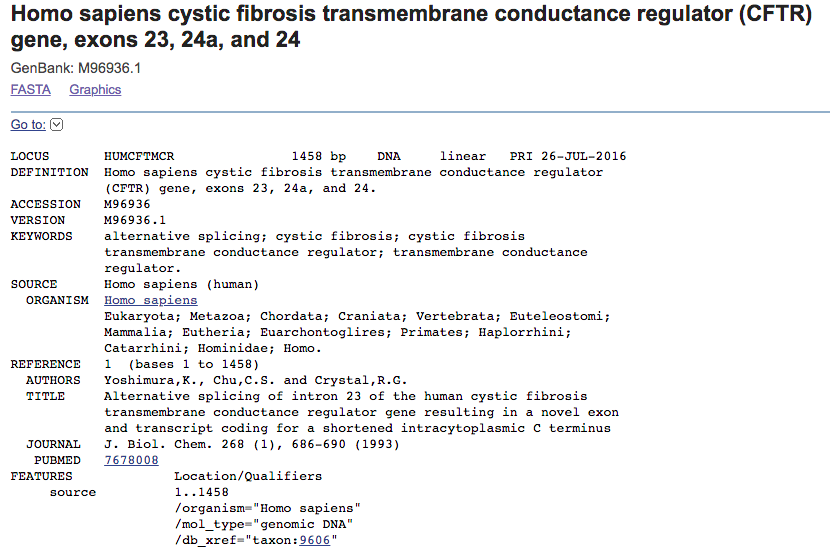
\includegraphics[scale=.4]{graphics/genbank.png}
	\end{center}
	\caption{A Genbank record comes from PubMed and contains contains diverse information for each known DNA sequence.}
	\label{fig:genbank}
\end{figure}


\vspace*{-.1in}
\subsubsection*{GitHub starter link}
\vspace*{-.1in}

\begin{center}
\color{red} \url{https://classroom.github.com/a/aDNdN-Ed} \color{black}
\end{center}


To use this link, please follow the steps below.
\begin{itemize}
	\item Click on the link and accept the assignment.
	\item Once the importing task has completed, click on the created assignment link which will take you to your newly created GitHub repository for this lab.
	\item Clone this repository (bearing your name) and work on the practical locally.
	\item As you are working on your practical, you are to commit and push regularly. You can use the following commands to add a single file, you must be in the directory where the file is located (or add the path to the file in the command):
		\begin{itemize}
		\item {\tt git add -A}
		\item {\tt git commit -m ``Your notes about commit here''}
		\item {\tt git push}
	\end{itemize}

	Alternatively, you can use the following commands to add multiple files from your repository:
	\begin{itemize}
		\item {\tt git commit <}\emph{nameOfFile}\tt{> -m ``Your notes about commit here''}
		\item {\tt git push}
	\end{itemize}
\end{itemize}
%%%

Be sure to read the {\tt README.md} file in the GitHub Classroom repository for instructions on how to complete your first assignment.


\vspace*{-.1in}
\subsection*{Objectives}
\vspace*{-.1in}

\begin{itemize}
	\item To apply information from Genbank record files for analysis.
	\item To generate Python3 code to manipulate genetic sequences in a variety of ways and make basic comparisons between sequences.
	\item To modify your existing code (if you choose) from lab 3 to be able to load Genbank files to display information about transcription and translation, and to conduct a comparative analysis. 
\end{itemize}
	
	
%	\item To automate a pipeline for sequence analysis and mutation detection.
%	\item Understand the structure and orientation of string representations of DNA and protein sequences.
%	\item Gain experience with string manipulation in a chosen programming language and its application to DNA and protein sequence data.
%\end{itemize}

\begin{figure}[ht!]
	\begin{center}
	 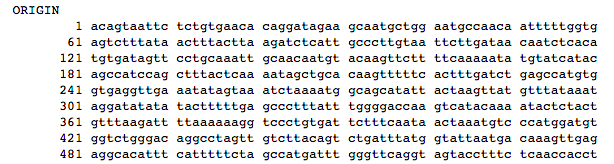
\includegraphics[scale=.4]{graphics/origin.png}
	\end{center}
	\caption{Each Genbank record has the DNA sequence data that can be placed into a {\tt FASTA} file.}
	\label{fig:origin}
\end{figure}



\vspace*{-.1in}
\subsection*{Developing Your Own Tool}
\vspace*{-.1in} 

	\subsubsection*{A Single tool for DNA mutation detection that loads data from Genbank files}
Comparisons between genetic material are extremely common in Bioinformatics. As discussed in class, the presence of alternative SNPs between samples of DNA, may help researchers to conclude whether a disorder can be expected from the organisms. Furthermore, mutations between code samples may also also serve to help researchers determine and potentially explain reasons for genetic abnormalities which may appear in protein formation, structure and, therefore, function. 

In this part of the lab you will develop a Python3 program that can manipulate sequences, transcribe and translate them and find mutations or general differences in sequences. Your working code that you are are to submit will be a modified version of the Python3 code (file: {\tt src/mutDetect\_i.py}) that you submitted for lab3's deliverable.



\vspace*{-.1in}
\subsubsection*{Required}
\vspace*{-.1in}

Please follow the below steps to create your Python3 program.

\begin{enumerate}
	\item Go to PubMed and download a single Genbank file of your choosing for a DNA record.
	\item Make a copy of the downloaded file and rename the copy's filename to include the word, {\tt mutation}. You are to manually edit this mutation file to include at least three (3) different types of mutations to the DNA (\emph{note: we discussed all these three mutations types in class}).
	\item Create a new Python3 program called: {\tt src/mutDetect\_ii.py}. You are welcome to use your solution from lab3's deliverable to begin this program however you will need to add the below functions and integrate their functionalities into you code.
	\item Functions to write;
	\begin{enumerate}

		\item \textbf{A function to load Genbank files}: The program must implement a function to load two Genbank files \emph{from steps 1 and 2, discussed above} and to isolate the DNA sequence material in each file using the BioPython library. You are free to chose how these files are loaded -- by command line inputs or by simply asking the user to enter filenames using an {\tt input()} function. 

		\item \textbf{A function to save FASTA files}: Your program must have a function to save a {\tt FASTA} file from each Genbank that is processed. 
	\end{enumerate}
	
	\item Once the DNA from each file has been obtained by parsing, your program is to transcribe and translate both DNA sequences to produce protein sequences (the function of the tool from the deliverable of lab3).
	\item After translation, your tool is to complete a comparison of the sequences, and to print out any differences found between both pairs of DNA, RNA and Protein. 
\end{enumerate}

\subsubsection*{Sample Output}

Your program should have an output that resembles the following;
\begin{center}\small
\begin{verbatim}
bioinformatics4Life$ ./mutDetect_ii.py <AnyKeyToStart>

	 Welcome to mutDetect_ii!
	 A program to compare DNA, make protein and compare protein sequences.

__Getting a Genbank sequence__
	 Enter the GenBank file name :wild.gb
	 Genbank record: M96936.1

__Writing a FASTA file__
	 Genbank record: M96936.1

__Getting a Genbank sequence__
	 Enter the GenBank file name :mut.gb
	 Genbank record: M96936.1

__Writing a FASTA file__
	 Genbank record: M96936.1
	 + Length of first sequence  : 1458
	 + Length of second sequence : 1458

__Comparing sequences__
	 + Seq char not the same at pos:  1
		 First seq char   :  C
		 Second  seq char :  T
	 + Seq char not the same at pos:  11
		 First seq char   :  C
		 Second  seq char :  G
	 + Sequences are same length:  True
	 
	  __Translation__
	 + Original DNA       : ACAGTAATTCTCTGTGAACACAGGATAGAAGCAATGCTG ... , length is : 1458
	 + PROTEIN from RNA   : TVILCEHRIEAMLECQQFLVSLYNFT*DLIALVILDNNLTCDSSCKLQQCTSSFQK
	 + protein1 sequence  : TVILCEHRIEAMLECQQFLVSLYNFT*DLIALVILDNNLTCDSSCKLQQCTSS ...
	 
 __Translation__
	 + Original DNA       : ATAGTAATTCTGTGTGAACACAGGATAGAAGCAATGCTGGAATGCCA, length is : 1458
	 + PROTEIN from RNA   : IVILCEHRIEAMLECQQFLVSLYNFT*DLIALVILDNNLTCDSSCKLQQCTSSFQK
	 + protein2 sequence  : IVILCEHRIEAMLECQQFLVSLYNFT*DLIALVILDNNLTCDSSCKLQQCTSS ... 
	 
 __Comparing sequences__
	 + Seq char not the same at pos:  0
		 First seq char   :  T
		 Second  seq char :  I
\end{verbatim}

\end{center}


\subsubsection*{Ethical Consideration: Questions in Blue}

Please read the National Public Radio article, \emph{U.S. Justice Department Charges 35 People In Fraudulent Genetic Testing Scheme} (link \url{https://www.npr.org/sections/health-shots/2019/09/27/765230011/u-s-justice-department-charges-35-people-in-fraudulent-genetic-testing-scheme}). You are to respond to the below \color{blue}\emph{Questions in Blue}\color{black}, shown below, which are also found in the Markdown file, {\tt ethical/reflections.md}, in your repository.

\color{blue}
	\begin{enumerate}
		\item What is the business incentive for the company (or the article) that prepared cancer-risk assessments for patients?

		\item Explain what practices were employed by the company?

		\item Which population did the company mentioned in the article target? In your opinion, why was this particular population chosen by the company?

		\item How were medical histories collected by doctors of the company? Comment on the ethical or unethical implications of the company's practices.

		\item According to the article, how was medical data collected for the cancer-risk assessment? In your opinion, what types of problems do you foresee happening as a result of the way that data was handled?

		\item Describe the technique used by the company in their feedback to patients. Comment on the ethical or unethical practices of their feedback method.
	\end{enumerate}
\color{black}

\vspace*{-.2in}
\subsubsection*{Required Deliverables}
\vspace*{-.1in}

\begin{itemize}
	\item Your completed activity should be saved as {\color{red} \tt src/mutDetect\_ii.py\color{black}} in the repository that you will push to GitHub.
	\item Please include your Genbank files (the one from the your download and the one that you edited to add the three (3) types of mutations.

	\item Ethical reflections:  Please respond to the reflection questions in the Markdown file, \color{red} {\tt ethics/reflections.md} \color{black} concerning the NPR article, \emph{U.S. Justice Department Charges 35 People In Fraudulent Genetic Testing Scheme}.

%    \item Write a reflection of about 100 words to describe your approach to finding the errors of the code. Record your reflection in the markdown document; {\tt \color{red} writing/reflections.md\color{black}}.	
	\end{itemize}

\noindent Please see the instructor if you have questions about the assignment submission.




\end{document}

%%%% junk bin %%%%%
%%%% junk bin %%%%%
%%%% junk bin %%%%%


%%%% start of my solution %%%%
#!/usr/bin/env python3

# Originally written by: Oliver Bonham-Carter
# email:
# Date: 13 Sept 2019
# Comment: A DNA translator and mutation detector.

# Library installation notes:
#
# Commands to install biopython
# python3 -m pip install biopython # global install
# python3 -m pip install biopython –user # local install

############################################################################
# TODO: In the other file, there are twelve bugs to fix. Did you find them?!
############################################################################


DATE = "29 Sept 2019"
VERSION = "i"
AUTHOR = " Oliver Bonham-Carter"
AUTHORMAIL = "obonhamcarter@allegheny.edu"

def help():
        h_str = "   "+DATE+" | version: "+VERSION+" |"+AUTHOR+" | "+AUTHORMAIL
        print("  "+len(h_str) * "-")
        print(h_str)
        print("  "+len(h_str) * "-")
        print("\n\tThe blank-blank program to do something cool.")
        #print("""\n\tLibrary installation notes:""")
        print("\t + \U0001f600  USAGE: python3 mutDetect_ii.py <any key to launch>")
        print("\t + Note: program requires two Genbank files.")
######################################################
#end of help()


def writeFastaFile(gbk_filename):
    """Function to create a fasta file from the GenBank file. Note: gbk_filename is a string of the Genbank filename"""
    print("\n__Writing a FASTA file__")
    #genbankfilename  filenames look like this --> "myGBfile-gb.fasta"
    faa_filename = gbk_filename.replace(".","-") + ".fasta"

    # open the files for working
    input_handle = open(gbk_filename,"r") # open file for reading (genbank input)
    output_handle = open(faa_filename,"w") # open file for writing (fasta output)

    # parse the genbank file for relevant information
    for seq_record in SeqIO.parse(input_handle, "genbank"):
        print("\t Genbank record: %s" % seq_record.id)
        output_handle.write(">%s %s\n%s\n" % (seq_record.id, seq_record.description, seq_record.seq))

    # close the files
    output_handle.close() # close the fasta file
    input_handle.close() # close the genbank file
# end of writeFastaFile()


def getGenbankSeq():
    """Function to load Genbank file and to extract the sequence"""
    print("\n__Getting a Genbank sequence__")
    prmpt = "\t Enter the GenBank file name :"
    gbk_filename = input(prmpt) # prompt the user to enter a filename for a genbank file

    # open file for reading (genbank input)
    input_handle = open(gbk_filename,"r")

    # parse the genbank file for relevant information
    seq = ""
    for seq_record in SeqIO.parse(input_handle, "genbank"):
        print("\t Genbank record: %s" % seq_record.id)
        #output_handle.write(">%s %s\n%s\n" % (seq_record.id, seq_record.description, seq_record.seq))
        seq = str(seq_record.seq)
    #print("\t Seq is ",seq, type(seq))

    # save the FASTA file.
    writeFastaFile(gbk_filename)

    # close the files
    input_handle.close() # close the fasta file

    return seq
# end of getGenbankSeq()


def getSeq():
    """ Function to get a sequence (a string) from the user"""
    print("\n__Getting a sequence__")

    prmpt = "\tEnter a sequence :"
    seq_str = input(prmpt)
    return seq_str.lower()

######################################################
# end of getSeq()


def compareSequences(seq1_str, seq2_str):
    """ Compares the sequences base by base"""
    print("\n__Comparing sequences__")

    for i in range(len(seq1_str)):
        # check to see whether the bases are the same going through the sequences
        try:
            if seq1_str[i] != seq2_str[i]: # are bases _not_ the same at the same position?
                print("\t + Seq char not the same at pos: ",i)
                print("\t\t First seq char   : ", seq1_str[i])
                print("\t\t Second  seq char : ", seq2_str[i])
        except IndexError:
            #print(" \t Sequences are uneven length!")
            pass
# end of compareSequences()

def getSeqLength(seq_str):
    """ Function to return the length of a sequence"""
    l_int = len(seq_str)
    if l_int % 3 != 0: # can we read triplets, groups of three?
        print("\t Warning! Sequence length cannot be divided into groups of triplets!")
    return l_int
######################################################
#end of getSeqLength()

def compareSeqLength(seq1_str, seq2_str):
    """Function to check the lengths of the sequences to make sure that they are the same length. This is necessary for making comparisons."""
    if len(seq1_str) != len(seq2_str):
        return False
    else:
        return True
######################################################
#end of compareSeqLength()

def translate(dna_str):
    """ Function to translate the DNA. Create a protein sequence from the DNA."""

    sequence = Seq(dna_str)
    #make some variables to hold strings of the translated code
    # give me RNA from the DNA
    RNAfromDNA_str = Seq.transcribe(sequence) #transcription step: converting dna to rna
    # give me DNA from the RNA
    DNAfromRNA_str = Seq.back_transcribe(sequence)
    # give me the protein from the dna
    PROTfromRNA_str = Seq.translate(RNAfromDNA_str)

    # print the output of the string variables
    print("\n__Translation__")

    print("\t + Original DNA       :", dna_str, ", length is :", len(dna_str))
    # print("\t + RNA from DNA     :", RNAfromDNA_str)
    # print("\t + DNA from RNA     :", DNAfromRNA_str)
    print("\t + PROTEIN from RNA   :",PROTfromRNA_str)

    return PROTfromRNA_str
######################################################
#end of translate()



def begin(task_str):
    """Driver function of program"""
    print("\n\t Welcome to mutDetect_ii!\n\t A program to compare DNA, make protein and compare protein sequences.")
# # get first DNA sequence
#     seq1_str = getSeq()
# # get second DNA sequence
#     seq2_str = getSeq()

#   get first DNA sequence from a GenBank file
    seq1_str = getGenbankSeq()

#   get second DNA sequence from a GenBank file
    seq2_str = getGenbankSeq()

    print("\t + Length of first sequence  :", getSeqLength(seq1_str))
    print("\t + Length of second sequence :", getSeqLength(seq2_str))

# compare the sequences
    compareSequences(seq1_str, seq2_str)
    print("\t + Sequences are same length: ",compareSeqLength(seq1_str, seq2_str))

    prot1_seq = translate(seq1_str)
    #print(type(prot1_seq))
    protein1_str = str(prot1_seq)
    print("\t + protein1 sequence  :",protein1_str)

    prot2_seq = translate(seq2_str)
    #print(type(prot2_seq))
    protein2_str = str(prot2_seq)
    print("\t + protein2 sequence  :",protein2_str)

    compareSequences(protein1_str, protein2_str)

######################################################
#end of begin()



import os, sys
#import math
# list other libraries below

# load my biopython library
from Bio.Seq import Seq
from Bio import SeqIO

if __name__ == '__main__':

        if len(sys.argv) == 2: # one parameter at command line
        # note: the number of command line parameters is n + 1
                begin(sys.argv[1])
        else:
                help() # If no command-line parameter entered, then run the help() function
                sys.exit()

%%%% end of my solution %%%%










